\subsection{Mô hình Bayesian Multinomial Logistic Regression}

Ta chỉ sử dụng vector đầu vào là vector gốc ban đầu làm đầu vào của mô hình

\subsubsection{Mô hình cho tập dữ liệu chỉ bao gồm các quan sát có cột "emailtotal" không phải giá trị null}

Ta có phân phối tiên nghiệm của mô hình:

\begin{python}
Intercept ~ Normal(mu: 0.0, sigma: 8.6712)
emailtotal ~ Normal(mu: 0.0, sigma: 2.5)
harass5_0 ~ Normal(mu: 0.0, sigma: 5.6887)
harass5_1 ~ Normal(mu: 0.0, sigma: 23.4185)
harass5_2 ~ Normal(mu: 0.0, sigma: 6.1126)
harass5_3 ~ Normal(mu: 0.0, sigma: 13.1386)
snapchat_0 ~ Normal(mu: 0.0, sigma: 5.0793)
snapchat_1 ~ Normal(mu: 0.0, sigma: 5.3936)
snapchat_2 ~ Normal(mu: 0.0, sigma: 8.3514)
instagrm_0 ~ Normal(mu: 0.0, sigma: 5.0793)
instagrm_1 ~ Normal(mu: 0.0, sigma: 5.5845)
instagrm_2 ~ Normal(mu: 0.0, sigma: 7.3225)
polviews_0 ~ Normal(mu: 0.0, sigma: 13.919)
polviews_1 ~ Normal(mu: 0.0, sigma: 13.4558)
polviews_2 ~ Normal(mu: 0.0, sigma: 7.0997)
polviews_3 ~ Normal(mu: 0.0, sigma: 7.2542)
polviews_4 ~ Normal(mu: 0.0, sigma: 5.205)
polviews_5 ~ Normal(mu: 0.0, sigma: 8.0149)
polviews_6 ~ Normal(mu: 0.0, sigma: 7.4671)
polviews_7 ~ Normal(mu: 0.0, sigma: 11.5643)
advfront_0 ~ Normal(mu: 0.0, sigma: 5.6802)
advfront_1 ~ Normal(mu: 0.0, sigma: 30.7027)
advfront_2 ~ Normal(mu: 0.0, sigma: 8.6656)
advfront_3 ~ Normal(mu: 0.0, sigma: 28.2596)
advfront_4 ~ Normal(mu: 0.0, sigma: 5.0861)
advfront_5 ~ Normal(mu: 0.0, sigma: 6.0088)
educ_2 ~ Normal(mu: 0.0, sigma: 71.8071)
educ_4 ~ Normal(mu: 0.0, sigma: 101.5197)
educ_5 ~ Normal(mu: 0.0, sigma: 101.5197)
educ_6 ~ Normal(mu: 0.0, sigma: 32.1914)
educ_7 ~ Normal(mu: 0.0, sigma: 45.4562)
educ_8 ~ Normal(mu: 0.0, sigma: 27.24)
educ_9 ~ Normal(mu: 0.0, sigma: 21.3111)
educ_10 ~ Normal(mu: 0.0, sigma: 15.177)
educ_11 ~ Normal(mu: 0.0, sigma: 12.9399)
educ_12 ~ Normal(mu: 0.0, sigma: 5.6152)
educ_13 ~ Normal(mu: 0.0, sigma: 8.6399)
educ_14 ~ Normal(mu: 0.0, sigma: 7.4671)
educ_15 ~ Normal(mu: 0.0, sigma: 10.9454)
educ_16 ~ Normal(mu: 0.0, sigma: 6.2904)
educ_17 ~ Normal(mu: 0.0, sigma: 12.3964)
educ_18 ~ Normal(mu: 0.0, sigma: 11.3668)
educ_19 ~ Normal(mu: 0.0, sigma: 16.2452)
educ_20 ~ Normal(mu: 0.0, sigma: 13.3474)
\end{python}

Do số lượng các tham số tương ứng rất lớn (khoảng hơn 300 tham số), nên ta sẽ thể hiện các tham số quan trọng tương ứng với các đặc trưng emailtotal, họ đặc trưng snapchat và instagrm.

\begin{figure}[H]
    \centering
    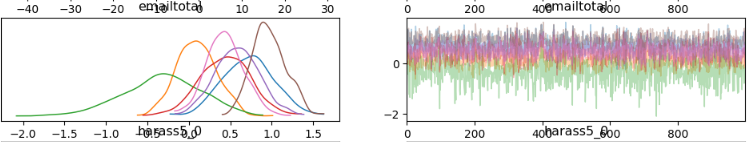
\includegraphics[width=0.8\textwidth]{figures/Thanh/Models/Bayesian_Multi_Logit/Bayesian_email_non_null_emailtotal_weights_plot.png}
    \caption{Hình vẽ biểu diễn phân phối hậu nghiệm các tham số tương ứng với đặc trưng emailtotal với các lớp khác nhau của cột wrkstat}
    \label{fig:Bayesian_email_non_null_emailtotal_weights_plot}
\end{figure}


\begin{figure}[H]
    \centering
    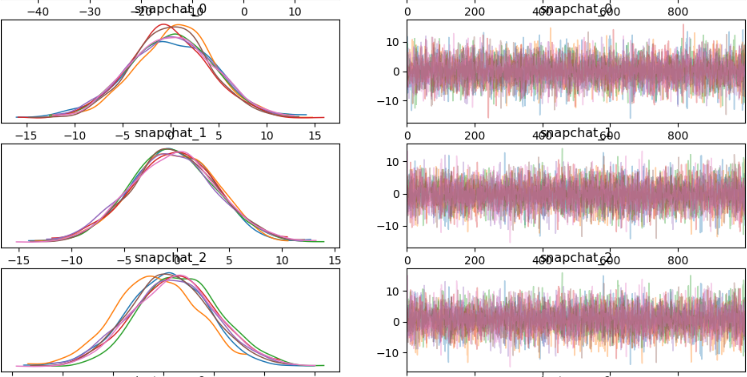
\includegraphics[width=0.8\textwidth]{figures/Thanh/Models/Bayesian_Multi_Logit/Bayesian_email_non_null_snapchat_weights_plot.png}
    \caption{Hình vẽ biểu diễn phân phối hậu nghiệm các tham số tương ứng với các đặc trưng của instagrm với các lớp khác nhau của cột wrkstat}
    \label{fig:Bayesian_email_non_null_snapchat_weights_plot}
\end{figure}

\begin{figure}[H]
    \centering
    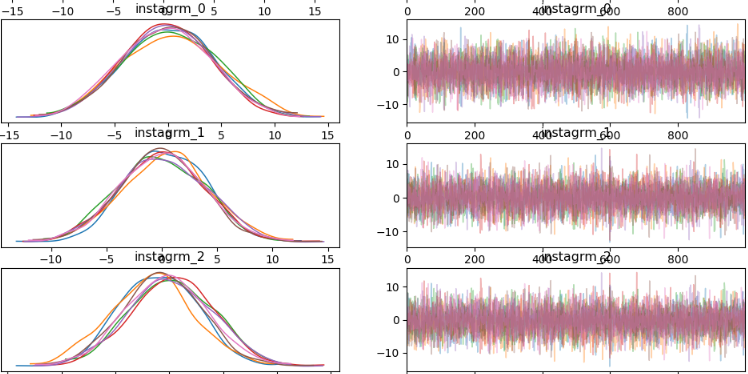
\includegraphics[width=0.8\textwidth]{figures/Thanh/Models/Bayesian_Multi_Logit/Bayesian_email_non_null_instagrm_weights_plot.png}
    \caption{Hình vẽ biểu diễn phân phối hậu nghiệm các tham số tương ứng với các đặc trưng của instagrm với các lớp khác nhau của cột wrkstat}
    \label{fig:Bayesian_email_non_null_instagrm_weights_plot}
\end{figure}

Các hình trên biểu diễn các phân phối hậu nghiệm của các tham số tương ứng với các đặc trưng emailtotal, họ đặc trưng snapchat và họ đặc trưng instagrm.
Ta nhận thấy các phân phối hậu nghiệm có dạng xấp xỉ phân phối chuẩn.

\begin{figure}[H]
    \centering
    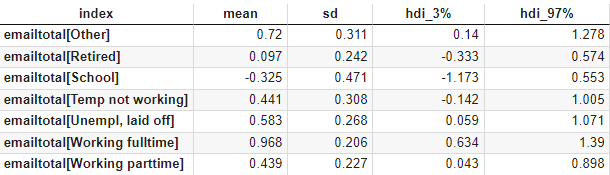
\includegraphics[width=0.6\textwidth]{figures/Thanh/Models/Bayesian_Multi_Logit/Bayesian_email_non_null_emailtotal_weights.png}
    \caption{Các phân vị mức và trung bình, độ lệch chuẩn của phân phối hậu nghiệm các tham số tương ứng với đặc trưng emailtotal}
    \label{fig:Bayesian_email_non_null_emailtotal_weights}
\end{figure}

\begin{figure}[H]
    \centering
    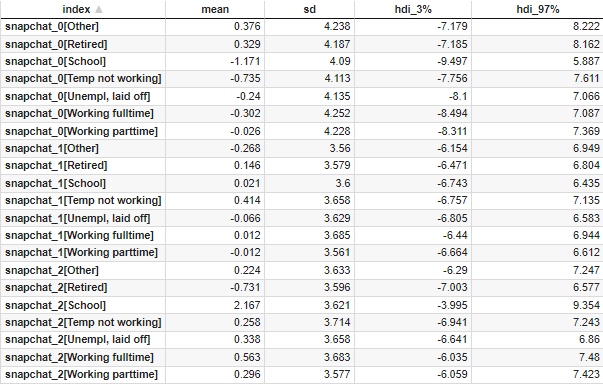
\includegraphics[width=0.6\textwidth]{figures/Thanh/Models/Bayesian_Multi_Logit/Bayesian_email_with_null_snapchat_weights.png}
    \caption{Các phân vị mức và trung bình, độ lệch chuẩn của phân phối hậu nghiệm của các tham số tương ứng với họ đặc trưng snapchat}
    \label{fig:Bayesian_email_with_null_snapchat_weights}
\end{figure}


\begin{figure}[H]
    \centering
    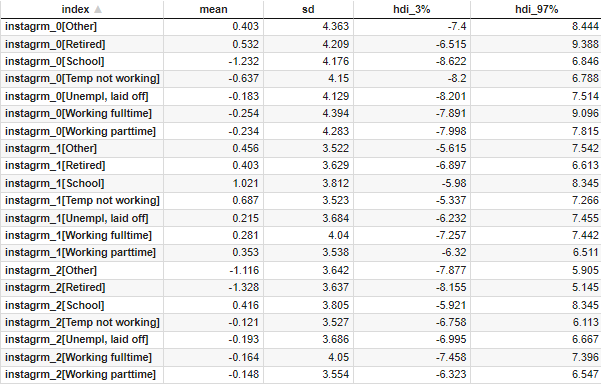
\includegraphics[width=0.6\textwidth]{figures/Thanh/Models/Bayesian_Multi_Logit/Bayesian_email_with_null_instagrm_weights.png}
    \caption{Các phân vị mức và trung bình, độ lệch chuẩn của phân phối hậu nghiệm của các tham số tương ứng với họ đặc trưng instagram}
    \label{fig:Bayesian_email_with_null_instagrm_weights}
\end{figure}

Ta nhận thấy độ lệch chuẩn của phân phối hậu nghiệm của các tham số tương ứng với đặc trưng emailtotal khá nhỏ.
Ngược lại độ lệch tiêu chuẩn của phân phối hậu nghiệm của các tham số tương ứng với họ đặc trưng snapchat và họ đặc trưng instagrm khá lớn trong khi trung bình lại khá nhỏ.
Nếu ta xét bài toán kiểm định trung bình của các tham số tương ứng với họ đặc trưng snapchat và họ đặc trưng instagrm có lớn hơn 0 hay không thì tiêu chuẩn thống kê khá nhỏ.
Điều này làm ta có kết luận sơ bộ những yếu tố sử dụng mạng xã hội snapchat hoặc instagrm không ảnh hưởng đến hình thức làm việc của một người.


